% Prof. Dr. Ausberto S. Castro Vera
% UENF - CCT - LCMAT - Curso de Ci\^{e}ncia da Computa\c{c}\~{a}o
% Campos, RJ,  2022
% Disciplina: An\'{a}lise e Projeto de Sistemas
% Aluno: Luiz Miguel Guedes Gomes

\chapterimage{planejamento.png} % Table of contents heading image
\chapter{Etapa de Planejamento}


Neste capítulo são abordados os motivos para implementação do sistema e os seus benefícios, seu orçamento, desenvolvimento do plano de trabalho e a viabilidade da instalação do sistema.


\section{Solicita\c{c}\~{a}o do Sistema}
%%%%%%%%%%%%%%%%%%%%%%%%%%%%%%%

\begin{itemize}
\item Responsável
	\begin{itemize}
	\item Luiz Miguel Guedes Gomes 
	\end{itemize}
\item Necessidade da empresa
	\begin{itemize}
	\item Este sistema visa suprir as demandas por facilidade, dinamismo e agilidade na gerência de redes especializadas na
comercialização de plantas, flores e produtos para jardinagem diretamente ao consumidor final, como hortos e floriculturas.
Através desse sistema, a gestão de estoque e de banco de dados se tornará muito mais precisa, e o atendimento ao cliente mais dinâmico e ágil, promovendo o aumento no número de vendas, evitando perdas de estoque, divulgando a marca da empresa, dinamizando sua relação com os fornecedores e melhorando na experiência do consumidor.
	\end{itemize}
\item Requisitos do Negócio
	\begin{itemize}
	\item O sistema será capaz de auxiliar na gestão de estoque, acusando possíveis perdas de mercadorias, indicando
oportunidades para serem realizadas promoções aos clientes, além de indicar a falta de produtos no estabelecimento.
	\item Será melhorado o gerenciamento sobre os bancos de dados, os quais conterão dados sobre estoque, vendas, encomendas, compra de insumos, despesas dos estabelecimentos, fornecedores, funcionários, clientes.
	\item Será capaz de gerar um relatório com o orçamento disponível para novas encomendas e gastos, o qual auxiliará na gestão do negócio e evitará preocupações com gastos excessivos e possíveis prejuízos.
	\item Também facilitará a realização de pedidos, compras e encomendas por parte dos clientes, por meio dos tablets distribuídos pelos setores que servirão para exibir produtos disponíveis, mostrar promoções e preços, descrição e cuidados com o produto, sendo também possível através deles realizar a compra ou a montagem de carrinhos de compra virtuais, que também contam com o recurso da montagem personalizada de encomendas.
	\item Será possível também, visualizar os produtos disponíveis, realizar a compra, encomenda e a montagem de carrinhos de compras virtuais de forma remota, através do aplicativo e do website, que podem ser entregues por frete ou retirada.
	\item A relação de produtos em falta e demandados pelos clientes será registrada no sistema e poderá ser fornecida aos fornecedores cadastrados, para que estes elaborem ofertas e orçamentos.
	\item As avaliações e os comentários sobre determinado produto feitos pelos clientes cadastrados poderá ser exibida, para incentivar a compra e a confiança de outros clientes sobre o produto oferecido.
	\item O sistema registrará quais são os produtos mais relevantes em um determinado período de tempo, podendo também realizar previsões de possíveis tendências no mercado, levando em consideração a estação do ano, datas festivas, entre outros aspectos, recomendando estes produtos aos clientes para que estes possam realizar compras e encomendas.
	\item O aplicativo no smartphone ou tablet do funcionário cadastrado, trará de forma unificada um arsenal de informações, opiniões, dados de estoque, preços e promoções acerca dos produtos que são de interesse ou serão oferecidos ao cliente.
	\item Sistema de detecção de entrada e saída de mercadorias do estabelecimento, para evitar furtos, desentendimentos, descontrole de dados de estoque, e implementar com segurança o sistema de autoatendimento.
	\end{itemize}
\item Valor agregado do sistema
	\begin{itemize}
	\item Valor tangível:
		\begin{itemize}
		\item Possibilitará com o recurso do melhoramento nos bancos de dados, uma maior precisão nas declarações de imposto 		de renda, desprendendo menos recursos para apurar esses dados e evitando pagamentos indevidos.
		\item Aumento no número de vendas. 
		\item Menor perda de estoque.
		\item Melhores ofertas por parte dos fornecedores e precisão nas encomendas.
		\end{itemize}
	\item Valor intangível:
		\begin{itemize}
		\item Com o auxílio dos métodos de autoatendimento, os funcionários serão menos sobrecarregados durante os horários		de pico de clientes, podendo assim desempenhar de forma mais dedicada o seu atendimento ao cliente, e se empenhar no			cuidado e na manutenção das mercadorias.
		\item O atendimento pessoal ao cliente será dinamizado e otimizado por meio do auxílio do aplicativo no smartphone ou
	tablet do funcionário. O que agilizará a venda e tornará esse funcionário disponível novamente para realizar outro atendimento.
		\item Crescimento do nome da marca, devido às inovações tecnológicas e principalmente no dinamismo, eficiência e
	dedicação no atendimento ao cliente.
		\end{itemize}
	\end{itemize}
\item Questões especiais e restrições
	\begin{itemize}
	\item O sistema deverá contar com um organizado esquema de hierarquia de cadastros, pois cada um fornecerá informações selecionadas ao seu usuário. Assim, clientes não poderão ver informações de funcionários e fornecedores, e fornecedores não poderão ver informações dos funcionários, da mesma forma, gerentes terão uma visão muito mais ampla sobre esses dados.
	 \item O sistema também deverá possuir um poderoso método de proteção de dados pessoais e comerciais dos seus usuários, não ferindo em nenhum aspecto as leis da LGPD.
	\item Para implantação desse sistema, deverá ocorrer treinamento e familiarização aos funcionários e novos contratados, para que todos os recursos desse novo sistema sejam usados em sua plena capacidade, extraindo assim, o máximo do potencial de todos envolvidos.
	\item Este sistema deverá também contar com uma interface de usuário de fácil acessibilidade e compreensão, assim como funcionário treinado para ensinar, caso preciso, o cliente ou fornecedor a como utilizá-lo. Desta forma, buscando abranger e atender a todos os tipos de pessoas, com suas dificuldades e diferentes necessidades.
	\end{itemize}
\end{itemize}

\section{Custos: Desenvolvimento e Operacional}
%%%%%%%%%%%%%%%%%%%%%%%%%%%%%%%

\begin{itemize}
\item Desenvolvimento 
	\begin{itemize}
	\item Salário das equipe e do pessoal do projeto
	\item Capacitação e instrução da equipe de desenvolvimento 
	\item Capacitação e instrução da equipe de antigos e novos funcionários
	\item Compra de hardwares e softwares
	\item Compra de mobílias e equipamentos para escritório 
	\item Compra dos equipamentos necessários para instalação do sistema de energia solar (opcional)
	\end{itemize}
\item Operacionais
	\begin{itemize}
	\item Salário de equipe operacional 
	\item Custo da instalação do novo sistema
	\item Custo da migração para o novo sistema
	\item Custo de atualização de softwares
	\item Custo de conserto e atualização de hardwares
	\item Custo de instalação e atualização dos serviços de comunicação 
	\item Custo de licenciamento de softwares proprietários
	\item Cobrança sobre os pacotes de internet contratados
	\item Custo da instalação do sistema de energia solar (opcional)
	\item Treinamento de novos usuários
	\end{itemize}
\end{itemize}

\section{Benef\'{\i}cios}
%%%%%%%%%%%%%%%%%%%%%%%%%%%%%%%


       \subsection{Benef\'{\i}cios Tang\'{\i}veis}
       	\begin{itemize}
	\item Reduções de pessoal 
	\item Otimização da manutenção de estoque
	\item Reduções de perda de estoque %tirar?
	\item Aumento nas vendas 
	\item Melhores preços de fornecedores 
	\item Maior controle sobre os dados do negócio %tirar?
	\item Otimização dos processos empresariais 
	\item Agilidade no atendimento aos clientes
        	\end{itemize}

       \subsection{Benef\'{\i}cios Intang\'{\i}veis}
	\begin{itemize}
	\item Aumento da fatia do mercado
	\item Aumento de reconhecimento da marca 
	\item Melhoria e dinamização no serviço voltado ao cliente
	\item Melhoria do uso do poder de decisão de compra do cliente 
	\item Aumento do bem estar no ambiente de trabalho 
	\item Melhores relações com fornecedores
	\item Aquisição de mercadoria com melhor qualidade
         	\end{itemize}

\section{An\'{a}lise de Custos e Benef\'{\i}cios}
%%%%%%%%%%%%%%%%%%%%%%%%%%%%%%%




\section{Estudo de Viabilidade}
%%%%%%%%%%%%%%%%%%%%%%%%%%%%%%%
Nessa seção serão apresentados o calendário e o cronograma das atividades a serem realizadas para a construção do sistema, assim como o cálculo do custo total do projeto, alternativas tecnológicas e recomendações importantes para o desenvolvimento do projeto. Com essas informações será possível chegar a uma conclusão sobre a viabilidade do projeto.

       \subsection{Calend\'{a}rio }
       \begin{table}[H]
	    \begin{center}
	    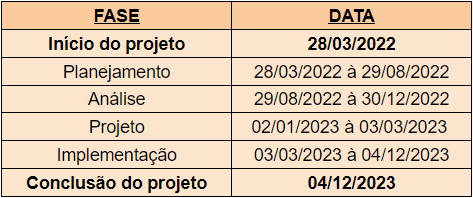
\includegraphics[width=12cm]{calendario.png}
	    \caption{Calendário com as fases do desenvolvimento do sistema} \label{tab:calend}
	    \end{center}
       \end{table} 

       \subsection{Cronograma }
       \begin{table}[H]
	    \begin{center}
	    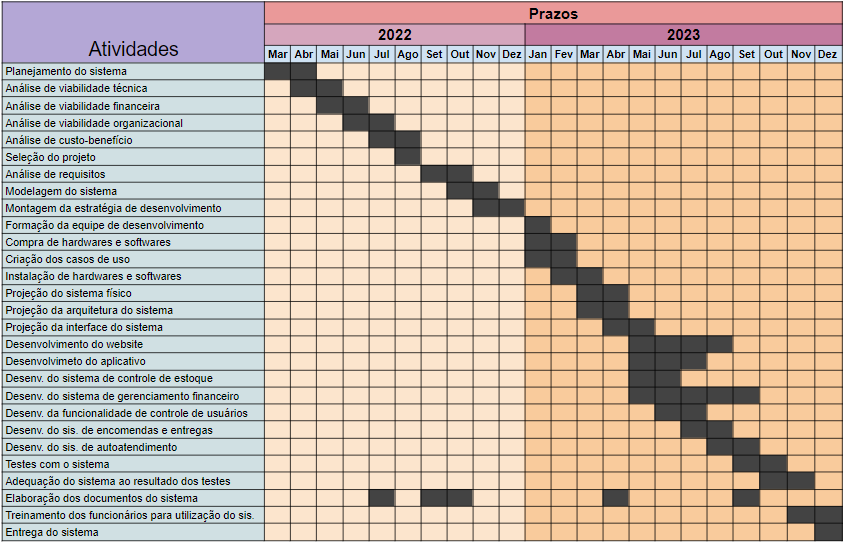
\includegraphics[width=16cm]{cronograma.png}
	    \caption{Cronograma das atividades para o desenvolvimento do sistema} \label{tab:crono}
	    \end{center}
       \end{table} 

       \subsection{Or\c{c}amento }
             \begin{table}[H]
	    \begin{center}
	    \includegraphics[width=14cm]{orçamento.png}
	    \caption{Orçamento do sistema} \label{tab:orca}
	    \end{center}
       \end{table} 

       \subsection{Alternativas Tecnol\'{o}gicas }
           Poderá ser incluído no orçamento a instalação de sistemas de energia solar com baterias para usar a energia excedente durante 		períodos noturnos, com o objetivo de reduzir o gasto com conta de energia fornecida pela concessionária e evitar a influência  de 	possíveis quedas na energia pública no funcionamento do sistema, de seus equipamentos e do servidor.	
	\begin{table}[H]
		    \begin{center}
		    \includegraphics[width=14cm]{orçamento_solar.png}
		    \caption{Orçamento opcional do sistema} \label{tab:orcaSol}
		    \end{center}
	\end{table} 
	


       \subsection{Recomenda\c{c}\~{o}es}
	\begin{itemize}
      \item Observar a possível alteração nos valores após período promocional dos pacotes de software assinados, devidamente salientados na tabela 2.3 e 2.4, e preferências por especificações de hardwares e softwares, para obter a melhor compatibilidade com o sistema previsto e não ter flutuações no orçamento elaborado. 
      \item O cronograma mostrado na tabela 2.2 deve ser devidamente seguido para que todos os equipamentos sejam adquiridos e todos os processos descritos sejam concluídos antes das datas comemorativas do mês de dezembro, e para isso deverá ocorrer a devida contratação de todos os funcionários descritos na seção "Pessoas" da tabela 2.3.
      \item A etapa de testes e de adequação aos mesmos é de suma importância para o sistema, pois o mesmo estará em constante interação com os usuários, e por isso deve funcionar corretamente e ser agradável ao uso.
	\end{itemize}
	\subsection{Conclusão de Viabilidade}
Após a análise sobre o cronograma das tarefas do sistema e sobre o seu orçamento, verifica-se que o mesmo atende às necessidades e não excede o orçamento estipulado pelo cliente. Sendo assim, conclui-se que o sistema de gerenciamento e tecnologização do comércio de flores e plantas: Pollinator é de fato viável do ponto de vista técnico, econômico e organizacional.
